\documentclass{article}
\usepackage{graphicx,spconf,amsmath,amssymb,subfigure,color}
\definecolor{darkgreen}{rgb}{0,0.5,0}
\newcommand{\Ntrg}{\big[N_{p=1, m=1} + \lambda \big] + \big[N_{p=1, m=2} + \lambda \big] + \ldots + \big[N_{p=1, m=M} + \lambda \big]}
\newcommand{\jointcnt}{\sum\limits_{n_{trg}=1}^{N_{trg}}I(X_p=x_p, X_{P-1}=x_{P-1})}
\newcommand{\singlecnt}{\sum\limits_{n_{trg}=1}^{N_{trg}}I(X_{P-1}=x_{P-1})}
\newcommand{\singlep}{p(X_{P-1}=x_{P-1})}
\newcommand{\singlepone}{p(X_{P-1}=1)}
\newcommand{\singleptwo}{p(X_{P-1}=2)}
\newcommand{\singlepM}{p(X_{P-1}=M)}
\newcommand{\condp}{p(X_p=x_p | X_{P-1}=x_{P-1})}
\newcommand{\jointp}{p(X_p=x_p, X_{P-1}=x_{P-1})}
\newcommand{\KmeansOuterSum}{\sum\limits_{k=1}^K}
\newcommand{\KmeansInnerSum}{\sum\limits_{{i=1 \atop x_i \in \mathcal{C}_k}}^N}
\newcommand{\KmeansSum}{\KmeansOuterSum \KmeansInnerSum}
\newcommand{\RVQInnerSum}{\sum\limits_{{i=1 \atop g_i \mapsto m_{\rho, s}}}^N}
\newcommand{\RVQOuterSum}{\sum_{m=1}^M}
\newcommand{\RVQsum}{\KmeansOuterSum \sum\limits_{{i=1 \atop g_i \in \mathcal{H}_k}}^N}
\newcommand{\KmeansInner}{{(x_i - y_k)}^2}
\newcommand{\RVQinner}{            {(x_i  - \hat{\mu}^{(k)})}^2}
\newcommand{\RVQinneralternate}{{(g_i - \mu_\rho^{(k)})}^2}
\newcommand{\RVQinneralternatealternate}{{(g_i - m_{\rho, s})}^2}
\newcommand{\KmeansError}{\KmeansSum \KmeansInner}
\newcommand{\RVQerror}     {\KmeansSum \RVQinner}
\newcommand{\RVQerroralternate}{\RVQsum \RVQinneralternate}
\newcommand{\RVQunit}{x_i -\bigg(\sum_{p=1}^P\mu^{(k)}_p\bigg)}
\newcommand{\RVQequivalentCodevector}{\sum_{p=1 }^P\mu^{(k)}_p}
\newcommand{\RVQequivalentCodevectorBroken}{\sum_{p=1 \atop p \neq \rho}^P\mu^{(k)}_p+ \mu^{(k)}_\rho}
\newcommand{\RVQmultipleKmeans}{x_i -\bigg(\RVQequivalentCodevectorBroken\bigg)}
\newcommand{\RVQmultipleKmeansone}{x_i -\bigg(\sum_{p=2}^P\mu^{(k)}_p+ \mu^{(k)}_\rho\bigg)}
\newcommand{\RVQmultipleKmeansonealternate}{\bigg(x_i -\sum_{p=1 \atop p \neq \rho}^P\mu^{(k)}_p\bigg) - \mu^{(k)}_\rho}
\newcommand{\RVQmultipleKmeanstwo}{x_i -\bigg(\sum_{p=1 \atop p \neq 2}^P\mu^{(k)}_p+ \mu^{(k)}_\rho\bigg)}
\newcommand{\RVQmultipleKmeansT}{x_i -\bigg(\sum_{p=1}^{P-1}\mu^{(k)}_p+ \mu^{(k)}_\rho\bigg)}
\newcommand{\EucMatrix}
{
\left[
\begin{array}{lll}
r_{11} & r_{12} & t_x \\ 
r_{21} & r_{22} & t_y \\ 
0 & 0 & 1 \\ 
\end{array}
\right]
}	

\newcommand{\SimMatrix}
{
\left[
\begin{array}{lll}
sr_{11} & sr_{12} & t_x \\ 
sr_{21} & sr_{22} & t_y \\
0 & 0 & 1 \\ 
\end{array}
\right]
}

\newcommand{\AffMatrix}
{
\left[
\begin{array}{lll}
a &b & t_x \\ 
c & d & t_y \\
0 & 0 & 1 \\
\end{array}
\right]
}

\newcommand{\ProjMatrix}
{
\left[
\begin{array}{lll}
h_{11} & h_{12} & h_{13} \\ 
h_{21} & h_{22} & h_{23} \\ 
h_{31} & h_{32} & h_{33} \\ 
\end{array}
\right]
}

\newcommand{\RotMatrixTheta}
{
\left[
\begin{array}{rr}
\cos(\theta) & -\sin(\theta) \\ 
\sin(\theta) & \cos(\theta) \\ 
\end{array}
\right]
}

\newcommand{\RotMatrixPhi}
{
\left[
\begin{array}{rr}
\cos(\phi) & -\sin(\phi) \\ 
\sin(\phi) & \cos(\phi) \\ 
\end{array}
\right]
}

\newcommand{\RotMatrixminusPhi}
{
\left[
\begin{array}{rr}
\cos(-\phi) & -\sin(-\phi) \\ 
\sin(-\phi) & \cos(-\phi) \\ 
\end{array}
\right]
}


\newcommand{\EigenvalueMatrix}
{
\left[
\begin{array}{cc}
\lambda_1 & 0\\
0 & \lambda_2
\end{array}
\right]
}

\newcommand{\bigMatrix}
{
s \left[
\begin{array}{cc}
 (r)(a) + b &  (r)(d) - c \\
 (r)(c) - d &  (r)(b) + a
\end{array}
\right]
}


\newcommand{\bigMatrixTwo}
{
\left[
\begin{array}{cc}
(\lambda_2) p + (\lambda_1) q & (\lambda_2) s  - (\lambda_1) r \\
(\lambda_2) r  - (\lambda_1) s & (\lambda_2) q + (\lambda_1) p
\end{array}
\right]
}
\newcommand{\dr}{(\mathbf{x}_i-\boldsymbol\mu_k)^T(\mathbf{x}_i-\boldsymbol\mu_k) + \lambda({P_{\textrm{max}}-P_i})}

\title{PCA Guided Fast Residual Vector Quantization For Processing Large Datasets}
\name{Salman Aslam}
\address{National University of Sciences and Technology, Islamabad, Pakistan\\salman@gatech.edu}	
\begin{document}
\ninept
\maketitle
\begin{abstract}
Residual Vector Quantization (RVQ) is a VQ method that has not gained much attention in the literature, first due to the difficulty of producing stable multi-stage designs, and second due to the computational complexity involved. Whereas the first problem has largely been solved, the second problem still limits wide usage of RVQ for processing large datasets. In this work, we introduce a novel method of implementing RVQ. This PCA guided method can be justified mathematically, results in simplifying the design process and greatly reduces the computational complexity required for RVQ design. As a result, large datasets can be efficiently compressed and retrieved in reasonable time.
\end{abstract}
%
\begin{keywords}
Residual vector quantization, RVQ, PCA
\end{keywords}

%########################################################################
\section{Introduction}
%########################################################################
RVQ is a powerful compression method first introduced by Juang et al.~\cite{1982_CNF_SpeechRVQ_JuangGray}.  The computational costs and memory requirements of regular Vector Quantization (VQ) are exponential in the data while both these requirements are linear for RVQ~\cite{1992_JNL_RVQ_Barnes}.  This feature makes RVQ attractive for processing large datasets.  In regular VQ, if 64 centroids are used, then intelligently using 64 centroids in an RVQ tree by placing them in 8 stages with 8 centroids per stage can lead to a total of $8^8=16,777,216$ terminal centroids!  The challenge of course is how to compute those 64 centroids.  The design procedure for multi-stage RVQ was developed by Barnes over several years~\cite{1996_JNL_AdvancesRVQ_Barnes}.  Since then, RVQ has been used for image coding~\cite{1992_CNF_ImageCodingRVQ_Kossentini} and more recently for image classification~\cite{2007_JNL_Katrina_Barnes, 2007_JNL_IDDM_Barnes}, target tracking~\cite{2012_CNF_PhD_Aslam} and for computing  classification error bounds~\cite{2013_THE_classRVQ_Irteza}.  


%########################################################################
\section{Quantization and RVQ}
%########################################################################


%---------------
\begin{figure}[h]	
\centering		
\fbox{
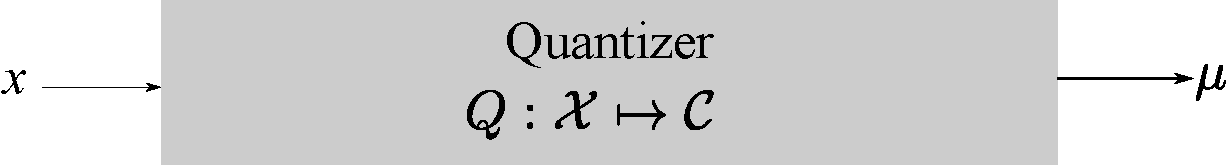
\includegraphics[width=0.3\textwidth]{figs/Quantization_blockDiagram.pdf}}
\caption{A quantizer $\mathcal{Q}$ maps symbols from a source alphabet $\mathcal{X}$ to symbols from a reconstruction alphabet $\mathcal{C}$, where in general, the number of elements in $\mathcal{X}$, $N >> K$, the number of elements in $\mathcal{C}$.}
\label{fig:Quantization_block_diagram}
\end{figure}
%---------------



Quantization is the process of representing a large, possibly infinite, set of values with a smaller set of values~\cite{2005_BOOK_DataCompression_Sayood}.  Figure~\ref{fig:Quantization_block_diagram} shows a quantizer $\mathcal{Q}$ that takes values from a source alphabet $\mathcal{X}=\{\mathbf{x} \in \mathbb{R}^D\}$ and maps them to a reconstruction alphabet $\mathcal{C}=\{\mathbf{y}_k \in \ \mathbb{R}^D \ | \ k=1,2, \ldots K\}$.  If the input is scalar, i.e. $D=1$, the quantizer is called a \emph{scalar quantizer}.  For $D>1$, the quantizer is called a \emph{vector quantizer}.  

The reconstruction alphabet $\mathcal{C}$ is known as the \emph{codebook} while the $K$ members $\mathbf{y}_k$ of the reconstruction alphabet $\mathcal{C}$ are called \emph{code-vectors}.  The term \emph{centroid} is used interchangeably with code-vector.  If we have $K$ code-vectors $\mathbf{y}_k$ in $\mathbb{R}^D$, $\log_2 K$ bits are required to represent each code-vector.   The \emph{resolution}, \emph{code rate}, or simply the \emph{rate} $r$ of a quantizer is the number of bits required to represent each sample, i.e., scalar element of $\mathbf{y}_k$.  Since there are $D$ samples, the rate $r=\frac{\log_2 K}{D}$.  

Figure~\ref{fig:quantization_scalar} illustrates the scalar quantization case for an input $X$ with distribution $f_X(x)$ and average distortion $e$,
\begin{equation}
\begin{array}{ll}
e &=\sum\limits_{k=1}^K \int\limits_{b_k}^{b_{k+1}}(x-y_k)^2f_X(x)dx
\end{array}
\end{equation}


%---------------
\begin{figure}[h]			
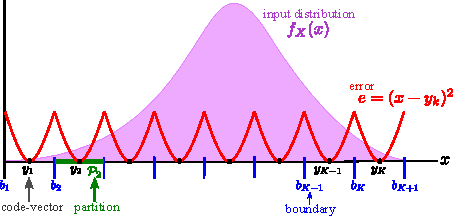
\includegraphics[width=0.45\textwidth]{figs/quantization_scalar.pdf}
\caption{Given partition $\mathcal{P}_k$, the optimal code-vector for this partition is the centroid of the partition.  Note that the reconstruction error increases exponentially as we move away from the centroids.}
\label{fig:quantization_scalar}	
\end{figure}
%---------------


In general, optimal coding of source vectors is not possible unless an exhaustive search over all code-vectors is carried out, as in structurally unconstrained \emph{Exhaustive Search Vector Quantizers} (ESVQs) \cite{1992_JNL_RVQ_Barnes}.  For a rate $r$ and dimension $D$, there are $K=2^{rD}$ code-vectors.  Therefore, the computational cost of ESVQ, $C_{ESVQ}$, and memory requirements $M_{ESVQ}$ are $\approx 2^{rD}$.  A solution to this problem is to impose constraints on the VQ structure.  One possible solution is the tree structured vector quantizer (TSVQ) proposed in~\cite{1980_JNL_TSVQ_Buzo}.  A $P$-level binary TSVQ has run-time search complexity which is only $C_{TSVQ} \approx 2P$ but double storage requirements, $M_{TSVQ} \approx 2 M_{ESVQ}$~\cite{1996_JNL_AdvancesRVQ_Barnes}.   So, although TVSQ solves the search complexity problem, it further aggravates the storage problem.  A method of reducing both run-time computational and storage complexity is to use a product code VQ~\cite{1991_BOOK_VQ_GershoGray}.  The basic idea in a product code VQ is to break a bigger problem into several smaller problems.  Examples include mean-residual VQ, gain-shape VQ, mean-gain-shape VQ and RVQ \cite{1996_JNL_AdvancesRVQ_Barnes}.  See~\cite{2011_THE_trkRVQ_Aslam} for a comparison of ESVQ, TSVQ and RVQ.

As with ESVQ and TSVQ, the $K$-means, or GLA, objective function to be minimized for RVQ for the discrete case can be written as,

\begin{equation}
e = \KmeansError
\label{eqn:RVQ_Kmeans_1}
\end{equation}																		


%---------------
\begin{figure}[t]
\centering	
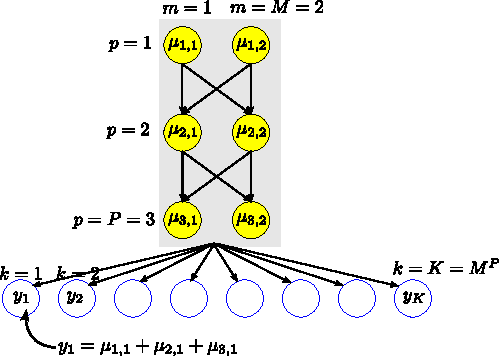
\includegraphics[width=0.45\textwidth]{figs/RVQ_trellis.pdf}
\caption{3x2 RVQ tree, 3 stages, 2 code-vectors per stage, i.e., $P$=3, $M=2$} 
\label{fig:RVQ_sigma_tree}				
\end{figure}
%---------------



%---------------
\begin{figure}[t]
\centering
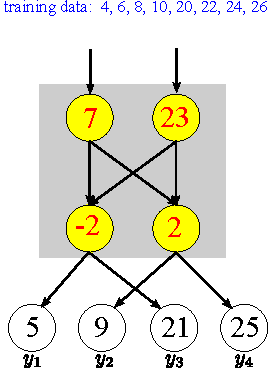
\includegraphics[width=0.3\textwidth]{figs/RVQ_introduction.pdf}
\caption{An example 2x2 RVQ tree.  In this case, 2 code-vectors in 2 stages, i.e. a total of 4 stage code-vectors lead to $2^2=4$ terminal code-vectors.}
\label{fig:RVQ_sigma_tree_example}
\end{figure}
%---------------



%---------------
\begin{figure}[t]
\centering
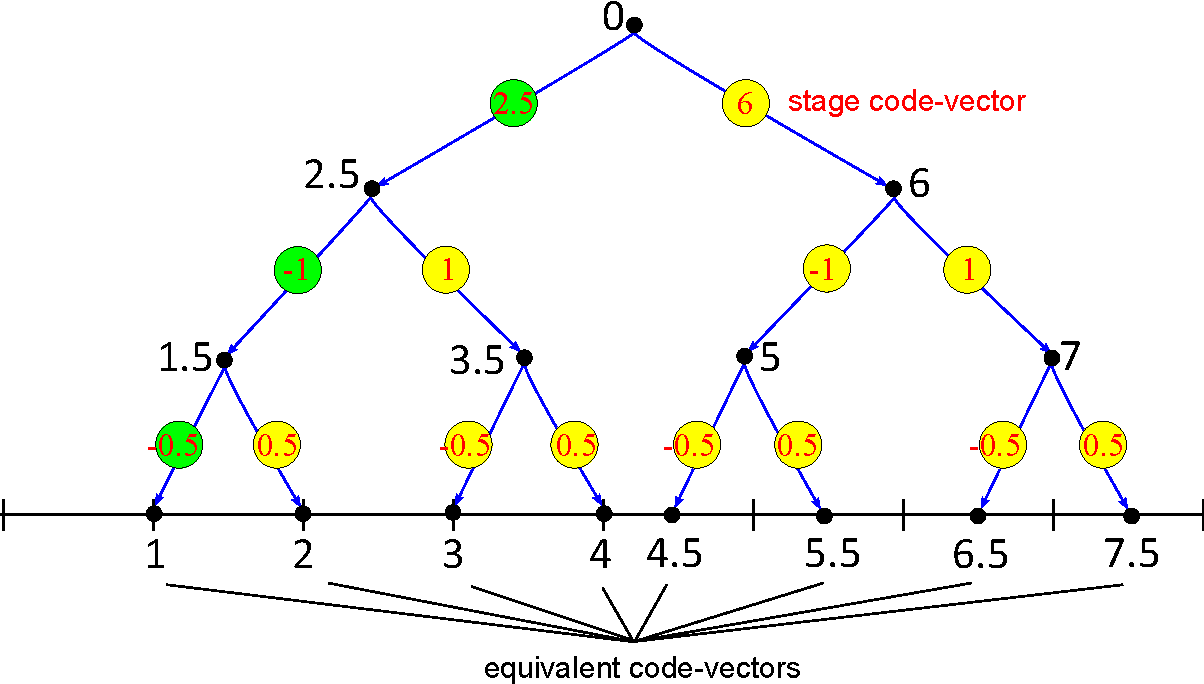
\includegraphics[width=0.5\textwidth]{figs/RVQ_trg_1_to_7_equivalentCVs.pdf}
\caption{In this example, the training data is \{1, 2, ... 7\} from which an RVQ tree is generated with 2.5 and 6 as first stage centroids, -1 and 1 as second stage centroids and -0.5 and 0.5 as third stage centroids.  At run time, the method shown is used to reconstruct the data points.}
\label{fig:RVQ_reconstruction}
%\subfigure[Entanglement using a 2x4 encoder codebook.]{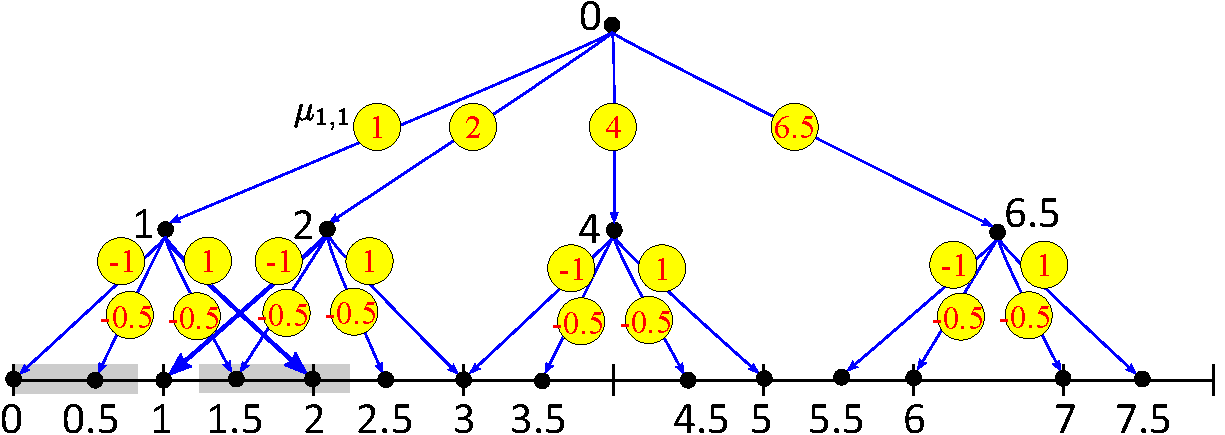
\includegraphics[width=0.75\textwidth]{figs/RVQ_trg_1_to_7_equivalentCVs_2.pdf}}
\end{figure}
%---------------



For RVQ, the $k$-th terminal code-vector is a direct sum of $P$ stage code-vectors, 

\begin{equation}
y_k = \mu_1^{(k)} + \mu_2^{(k)} + \ldots + \mu_P^{(k)}
\end{equation}

Substituting this notation in Equation~\ref{eqn:RVQ_Kmeans_1} and grouping all stage code-vectors except for the stage code-vector at the $\rho$-th stage gives us a series of equivalent equations, one equation per stage,

\begin{align}
e&= \KmeansSum{\bigg[\RVQmultipleKmeansone\bigg]}^2, \ \ \rho=1\notag\\
&= \KmeansSum{\bigg[\RVQmultipleKmeanstwo\bigg]}^2, \ \ \rho=2\notag\\
&\ \ \ \  \ \ \ \vdots\notag\\
&=\KmeansSum{\bigg[\RVQmultipleKmeansT\bigg]}^2, \ \ \rho=P
\label{eqn:RVQ_Kmeans_2}
\end{align}

Equation~\ref{eqn:RVQ_Kmeans_2} can be regrouped and written in compact notation as,

\begin{align}
e&= \KmeansSum{\bigg[\RVQmultipleKmeansonealternate\bigg]}^2, \ \ \rho=\{1, 2, \ldots P\}\notag\\
&={\RVQerroralternate}, \ \ \rho=\{1, 2, \ldots P\}
\label{eqn:RVQ_Kmeans_3}
\end{align}																



where $g_i$ is the \emph{graft residual}~\cite{1993_JNL_RVQDSC_Barnes}.   As can be seen in Equation~\ref{eqn:RVQ_Kmeans_3}, the graft residual $g_i$ for a data-point $x_i$ is formed by subtracting from $x_i$, all stage codevectors that are used to reconstruct $x_i$ except the stage codevector at the $\rho$-th stage.  In this sense, $g_i$ is a causal anti-causal (CAC) residual~\cite{1993_JNL_RVQDSC_Barnes}.  The code-vectors at the $\rho$-th stage are computed using the $K$-means objective function for that particular stage.  The implication of this step is that the RVQ objective function is now a coupled $K$-means objective function where the design of each stage code-vector depends on stage code-vectors from all other stages, and not just prior stages, hence the name causal anti-causal.    A challenge in this coupled $K$-means setup is that computing the centroids for one stage changes the residual centroids for all other stages.  

An RVQ is different from a traditional VQ in the sense that it partitions the input space $\mathbb{R}^D$ into $M$ cells.  The residual space, also in $\mathbb{R}^D$, is then partitioned again into $M$ cells.  This process is repeated $P$ times.  The advantage of this approach is that in obtaining $M^P$ partitions, we need to run our partitioning algorithm $P$ times and generate $M$ partitions at each stage.  In traditional VQ, the partitioning algorithm would run once but have to create $M^P$ partitions.  For the binary case (two code-vectors per stage, $M=2$) and a total of 8 stages ($P$=8), RVQ only requires 16 searches.  In $ESVQ$, this would require 256.  The exponential complexity is reduced to linear complexity.  In general, structurally constrained quantizers cannot provide performance as good as ESVQ.  However, since they are able to more efficiently implement codes, larger and larger vector sizes can be used, and if carefully designed, can achieve better performance that ESVQ for a given computational cost~\cite{1996_JNL_AdvancesRVQ_Barnes}.  The general form for an RVQ tree is given in Figure~\ref{fig:RVQ_sigma_tree} while an example RVQ tree is given in Figure~\ref{fig:RVQ_sigma_tree_example}.  In Figure~\ref{fig:RVQ_reconstruction} RVQ reconstruction procedure at run-time is shown while Figure~\ref{fig:RVQ_2Dtree} displays the nature of an RVQ tree when used with images.






%---------------
\begin{figure}[t]
\centering\subfigure[Snapshots from image sequence taken from~\cite{2008_JNL_subspaceTRK_Ross}.]{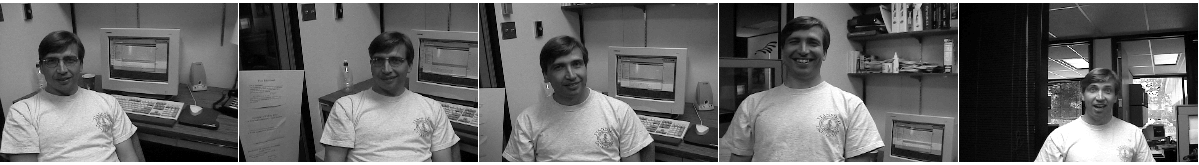
\includegraphics[width=0.45\textwidth]{figs/seq_1_Dudek.png}\label{fig:trk_pca_1a}}
\subfigure[An 8x4 RVQ tree created from the dataset given above.]{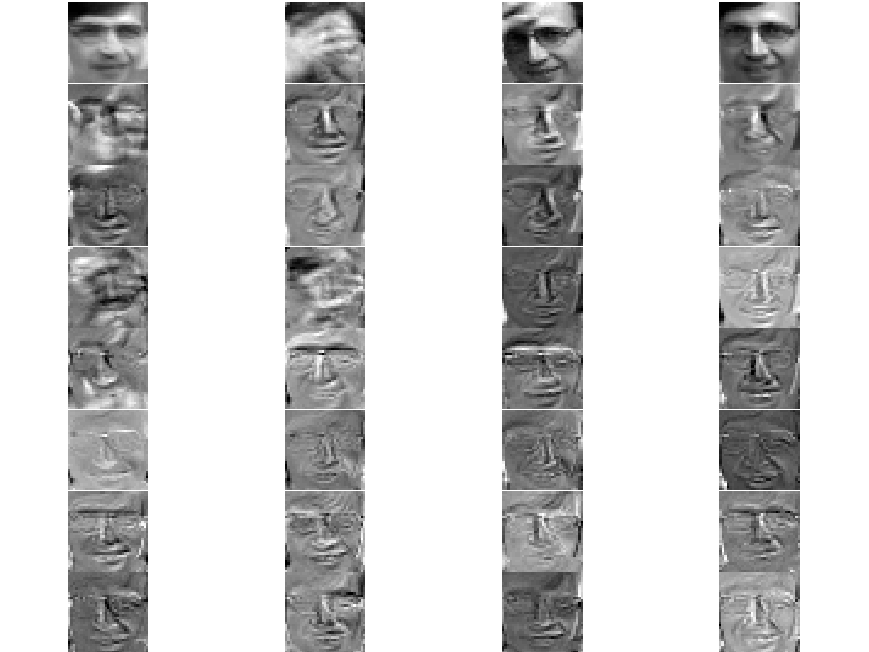
\includegraphics[width=0.45\textwidth]{figs/1_Dudek__aRVQ_08_04_1000_0_RofE__170_codebook.pdf}
}
\caption{In this example, we show what an RVQ tree looks like for 2D data.}
\label{fig:RVQ_2Dtree}
\end{figure}
%---------------








%########################################################################
\section{PCA Guided RVQ}
%########################################################################
Having taken care of the preliminaries, we are interested in the relationship between PCA and RVQ.  The reason is both academic and practical.  From an academic point of view, it is inherently satisfying to be able to relate a less known algorithm with a widely known one.  Additionally, many existing results may become relevant for the new algorithm.  In this context, the work by Ding and He~\cite{2004_CNF_KmeansVsPCA_DingHe} of relating PCA to the $K$-means algorithm is particularly relevant since we have already shown that RVQ is based on coupled $K$-means.  From a practical standpoint, relating RVQ to PCA greatly simplifies the the complex and heuristic design process of RVQ and leads to great reductions in computational complexity.

In this context, we are interested in the following two questions:
\begin{enumerate}
\item PCA generates the centroid cluster subspace $S$ while RVQ generates stage subspaces, $S_1, S_2, \hdots, S_P$, one stage subspace for each of the $P$ stages.  What is the relationship between the subspace generated by PCA and the subspaces generated by RVQ?
\item PCA generates eigenvectors of the data while RVQ generates stage centroids.  What is the relationship between the eigenvectors and the stage centroids?
\end{enumerate}
% lie in subspace $T$.  
In order to answer the first question, we note that according to Ding and He~\cite{2004_CNF_KmeansVsPCA_DingHe}, if we ran the $K$-means algorithm on the $N$ input data points $x_i~\in~R^D, K<D, i=1, 2, \hdots N$, the resulting $K$ equivalent centroids, $y_k$, would lie in cluster centroid subspace $S$ with dimensionality $K~-~1$.  Now, if we ran RVQ on this input data, the stage centroids $\mu_{m,p}$ would add up in $K=M^P$ different combinations to make the equivalent centroids $y_k$.  Quite clearly, the equivalent centroids $y_k$ are linear combinations of the stage centroids.  Therefore, the stage centroids must also lie in $S$.  Furthermore, the $M$ stage centroids at a particular stage lie in a subspace whose dimensionality is at most $M-1$.  Therefore, stage centroids in the first stage, i.e, $p=1$ lie in $M-1$ dimensional stage subspace $S_1$, stage centroids in the second stage, i.e, $p=2$ also lie in $M-1$ dimensional stage subspace $S_2$, and so on till $P$ stages.  Therefore, $S_1, S_2, \hdots, S_P \subset S$.

In order to answer the second question, we again turn to Ding and He in that PCA dimension reduction automatically performs data clustering according to the $K$-means objective function~\cite{2004_CNF_KmeansVsPCA_DingHe}.  For PCA, data reconstruction error is minimized if the data is represented in the $K-1$ lower dimensional subspace as projections onto the principal directions $\mathbf{u}_k$ where $YY^T\mathbf{u}_k=\lambda_k\mathbf{u}_k$.  $y_i$ is the zero-mean version of the input data $x_i$, $Y$ is the zero-centered input matrix formed from the data $y_i$ and $\lambda$'s are the eigenvalues.  If $K$-means clustering is to be carried out in the PCA subspace as suggested by~\cite{2004_CNF_KmeansVsPCA_DingHe} , then RVQ stage centroids placed in this subspace must be placed so that they account for maximum variance in the data.  This will happen if they are placed on the eigenvectors generated by PCA.  A vector sum of these stage centroids will then account for maximum variance in the data.  If the data residual from one stage still has more variance than the data's variance in an orthogonal direction, then repeated application of this rule will place subsequent stage centroids along the same eigenvectors until the residual data's variance falls below the variance in an orthogonal dimension.  In summary, stage centroids from one stage to another will either lie along the same eigenvector, or along an orthogonal eigenvector.  This is illustrated using a simple example in Figure~\ref{fig:PCAguidedRVQ_simpleExample}.  

In this example, the input data consists of two elliptically shaped clusters whose variance is greatest along the x-axis.  Optimal fist stage centroids are placed on the prinicipal direction, i.e., the x-axis.  The variance of the residual data, i.e, input data from which the corresponding centroids have been subtraced also has maximum variance along the x-axis.  Second stage optimal centroids are also therefore placed along this dimension.  This process repeats for the third stage as well and once again, optimal third stage centroids lie along the x-axis.  Finally, in the fourth stage, the variance along the orthogonal direction, the second PCA eigenvector, i.e, y-axis is now greater than along the x-axis and therefore optimal fourth stage centroids now lie along the y-axis. 


%---------------
\begin{figure}[t]
\subfigure[Stage 1.  The two first stage centroids lie on the principal eigenvector, $x$-axis in this case, accounting for maximum variance.]{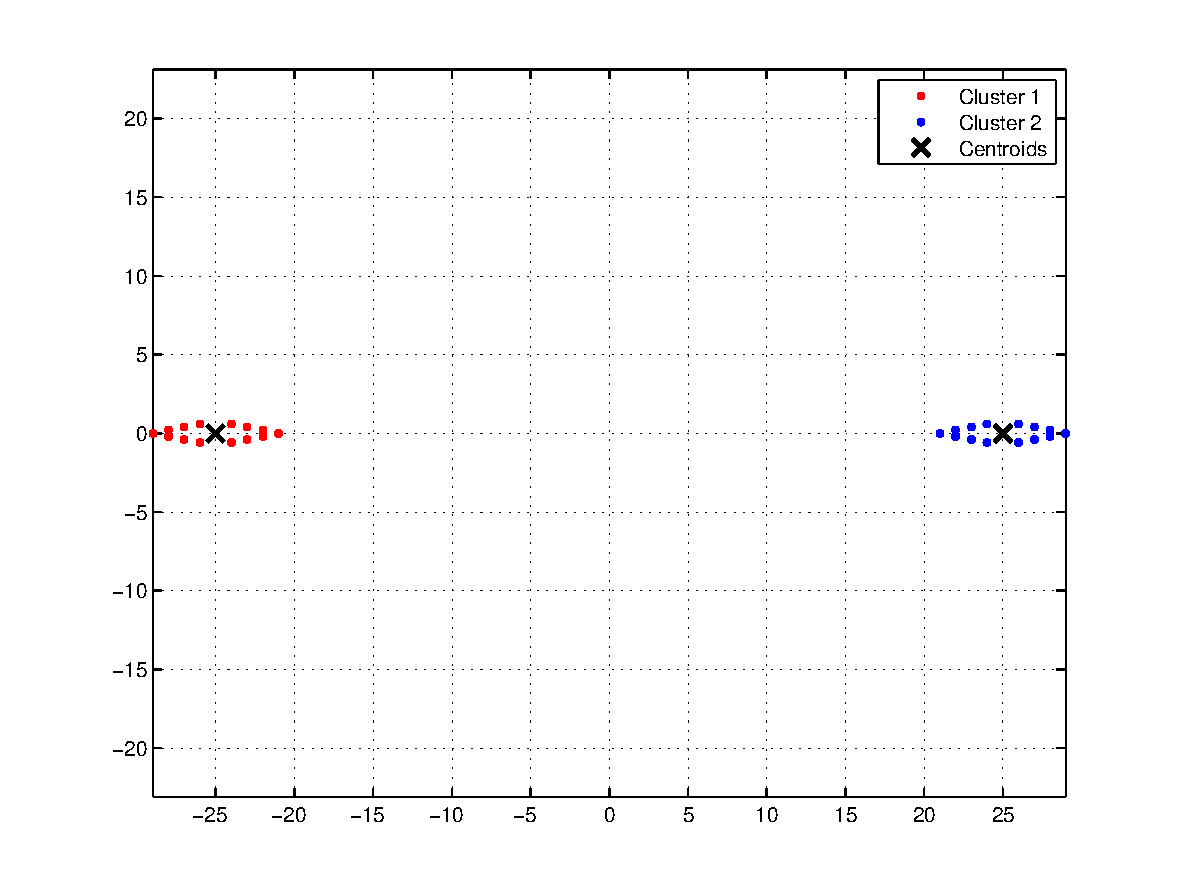
\includegraphics[width=0.25\textwidth]{figs/PCAguideRVQ1.pdf}}
\hspace{0.1in}\subfigure[Stage 2.  The data points here are the residuals from stage 1.  Notice that the variance along the principal eigenvector is still more than the variance in the orthogonal direction.  Therefore, the stage centroids of the second stage also lie along the principal eigenvector.]{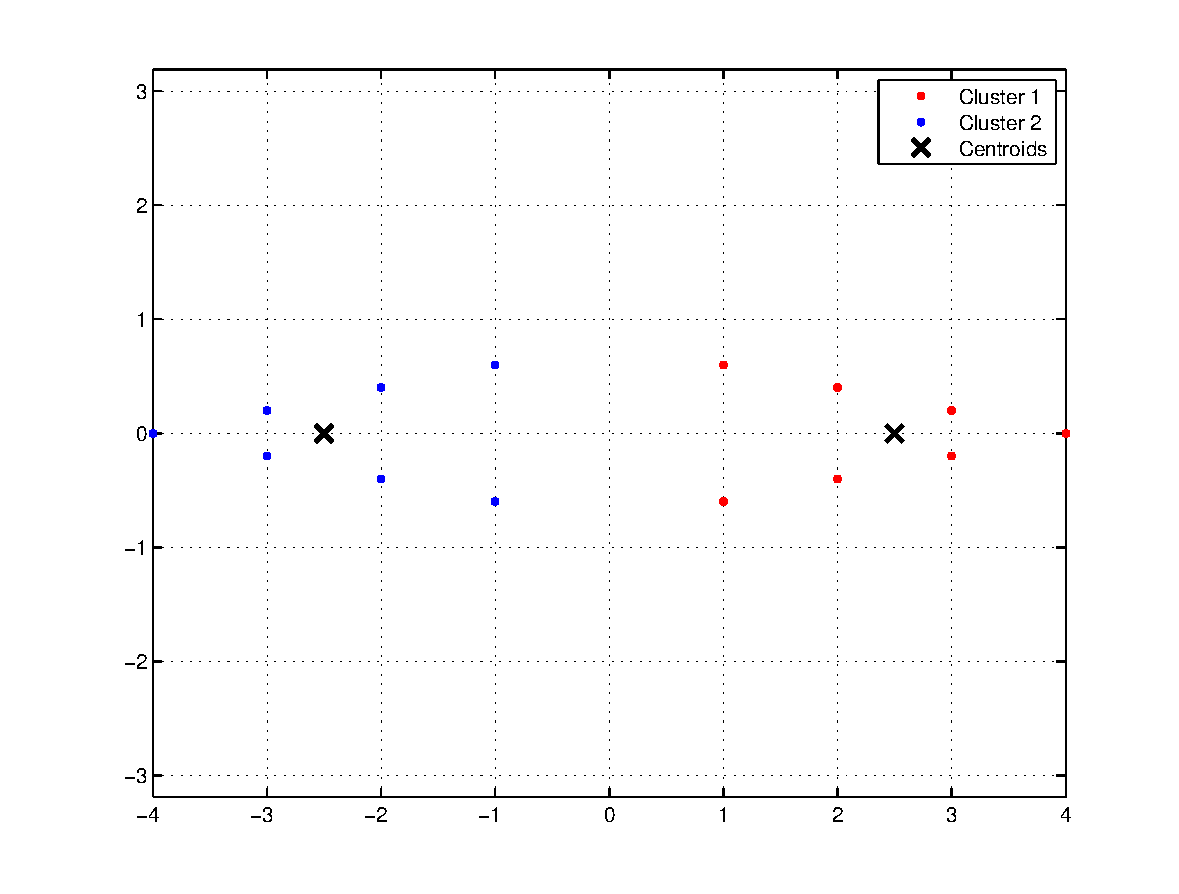
\includegraphics[width=0.25\textwidth]{figs/PCAguideRVQ2.pdf}}\\
\subfigure[Stage 3.  As in stage 2, the variance along the principal direction is still greater than the variance in the orthogonal direction, and therefore once again, the stage centroids lie on the principal eigenvector.]{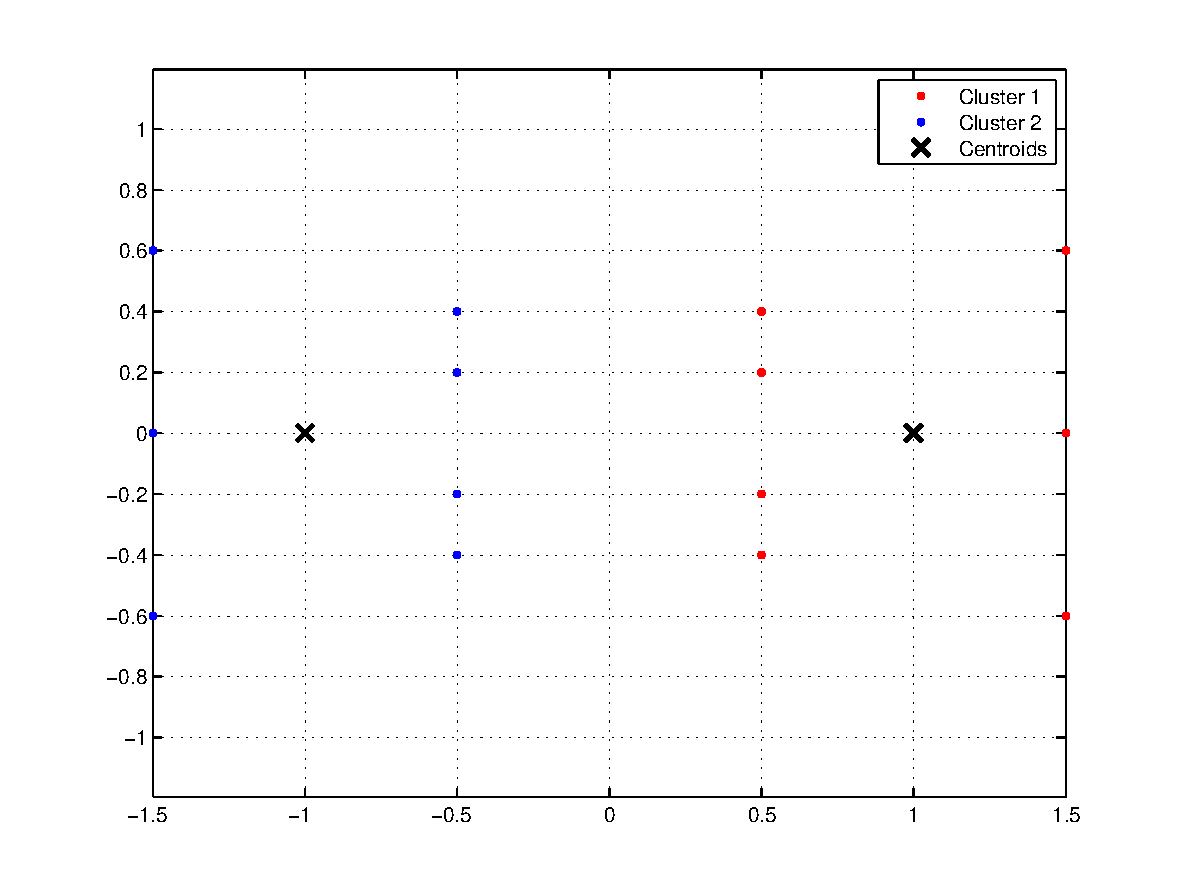
\includegraphics[width=0.25\textwidth]{figs/PCAguideRVQ3.pdf}}
\hspace{0.1in}\subfigure[Stage 4.  Finally, the variance in the principal direction is less than in its orthogonal direction, and therefore the stage centroids at this stage are aligned along the orthogonal direction.]{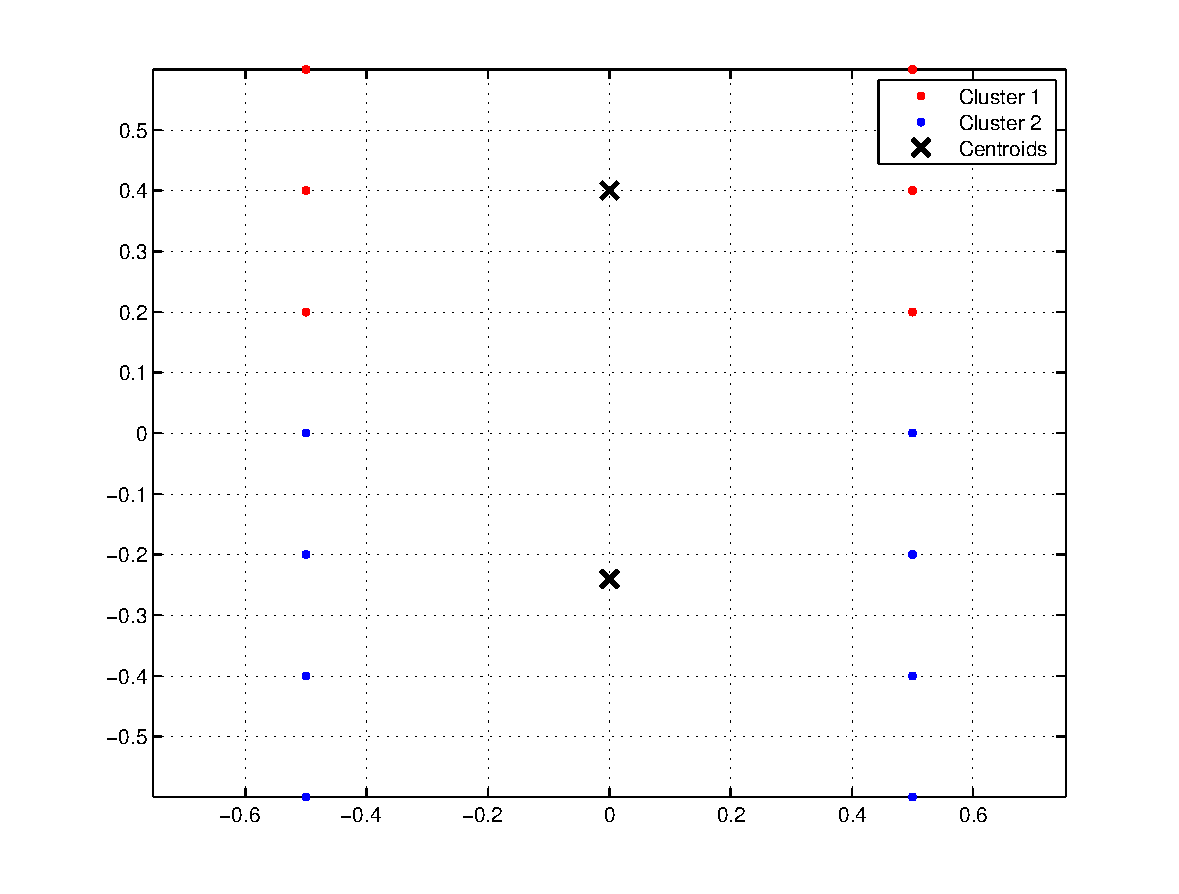
\includegraphics[width=0.25\textwidth]{figs/PCAguideRVQ4.pdf}}
\caption{PCA guided RVQ.  A simple example in $\mathbb{R}^2$.  Each data point given in the top left figure is reconstructed using a sum of stage centroids, one from each stage.  Notice the decreasing variance of the residual data as each stage progresses (evident from less spread along the x-axis).} 
\label{fig:PCAguidedRVQ_simpleExample}
\end{figure}
%---------------




%########################################################################
\section{Conclusions}
%########################################################################
RVQ holds tremendous potential for representing large datasets in compact notation.  For instance, an 8x8 RVQ with 8 stages and 8 stage centroids per stage for a total of 64 centroids actually has  $8^8=16,777,216$ terminal centroids.  Despite the large compression ratios possible, RVQ has not found widespread usage.  The reason is the difficulty in its design.  In this work, we have attempted to extend the relationship between PCA and $K$-means to PCA and RVQ resulting in considerably lower design complexity.  We have also provided a theoretical justification for this design process.  Currently, we are evaluating this design methodology on larger datasets. 





%In other words, PCA finds the most discriminative subspace and clustering carried out in this subspace 


%However, if each data point is to be represented by a centroid rather than by its projection, the reconstruction error will be minimum if the centroid lies within the PCA subspace.  The reason is that PCA minimizes the reconstruction error and using a centroid outside this subspace will only add a component to the error.  Argument against this: PCA is a linear transformation, so you cannot say that its reconstruction error is best.  It is best among all linear transformations, but clustering is non-linear.

%An alternate way of looking at this is to say that both PCA and RVQ transform the input data $x_i$ in different ways.  Whereas PCA is applied on the zero-centered data $y_i$, RVQ is applied on the graft residuals $g_i$ 
 

\bibliographystyle{IEEE}
\bibliography{MyCitations}
\end{document}
